\documentclass{article}

\usepackage{amsmath, graphicx, makecell}
\graphicspath{ {./images/} }

\begin{document}

\section*{Ch. 14 CW \#1 Solutions}

\begin{enumerate}

\item In the long run, firms' ATC curves are a flatter U-shape and lie below their short run ATC curves. That's because in the long run there are no fixed costs -- all costs are variable. As a result, firms have more flexibility to choose their inputs and keep their costs low.

\item (a) -- Specialization makes workers more productive, so their marginal product increases. That means the firms ATC will decrease as they produce more, so it will exhibit economies of scale.

\item (d) -- As production increases, average total cost increases. That means Boeing exhibits diseconomies of scale. 

\item

	\begin{enumerate}
	
	\item Its fixed cost is \$300.
	
	\item Marginal cost is the same regardless of whether you calculate it as the change in total cost or the change in variable cost. That's because fixed cost doesn't change when we increase output by one, so the change in total cost is entirely the change in variable cost. Mathematically,
	
	\begin{align*}
	\Delta TC &= TC_2 - TC_1 \\
	&= (FC + VC_2) - (FC + VC_1) \\
	&= VC_2 - VC_1 \\
	&= \Delta VC
	\end{align*}
	
	\begin{center}
	\begin{tabular}{c | c | c | c | c}
	Quantity & TC & VC & $MC = \Delta TC$ & $MC = \Delta VC$ \\
	\hline
	0 dozen pizzas & \$300 & \$0 & -- & -- \\
	1 & 350 & 50  & 50 & 50 \\
	2 & 390 & 90 & 40 & 40 \\
	3 & 420 & 120 & 30 & 30 \\
	4 & 450 & 150 & 30 & 30 \\
	5 & 490 & 190 & 40 & 40 \\
	6 & 540 & 240 & 50 & 50 \\
	\end{tabular}
	\end{center}
	
	\end{enumerate}
	
\item The efficient scale of the company is 4 houses painted per month. 

	\begin{center}
	\begin{tabular}{| c | c | c | c | c | c | c | c |}
	\hline
	\makecell{Quantity of\\Houses\\Painted per\\Month} & 1 & 2 & 3 & 4 & 5 & 6 & 7 \\
	\hline
	\makecell{Variable\\Costs} & \$10 & \$20 & \$40 & \$80 & \$160 & \$320 & \$640 \\
	\hline
	$AFC = \frac{FC}{Q}$ & 200 & 100 & 66.67 & 50 & 40 & 33.33 & 28.57 \\
	\hline
	$AVC = \frac{VC}{Q}$ & 10 & 10 & 13.33 & 20 & 32 & 53.33 & 91.43 \\
	\hline
	$ATC$ & 210 & 110 & 80 & 70 & 72 & 96.67 & 120 \\
	\hline
	\end{tabular}
	\end{center}
	
\item

	\begin{enumerate}
	
	\item A lump-sum tax is a single payment that every person or firm (or in this case every hamburger firm) has to pay. A lump-sum tax is a fixed cost, so the average fixed cost and average total cost curves shift. Marginal cost doesn't shift because marginal cost just depends on variable cost (as we saw in 4).

		\begin{center}
		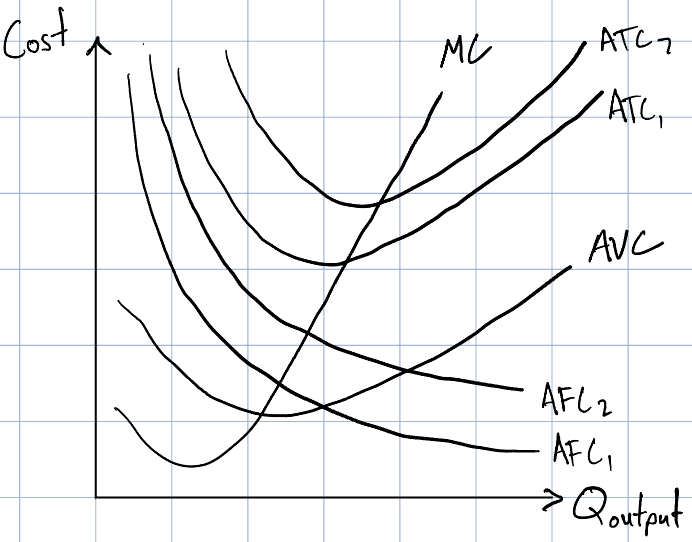
\includegraphics[width = 0.5\textwidth]{p6a}
		\end{center}
	
	\item The per-burger tax is a variable cost, so the average variable cost, average total cost, and marginal cost curves shift.
	
		\begin{center}
		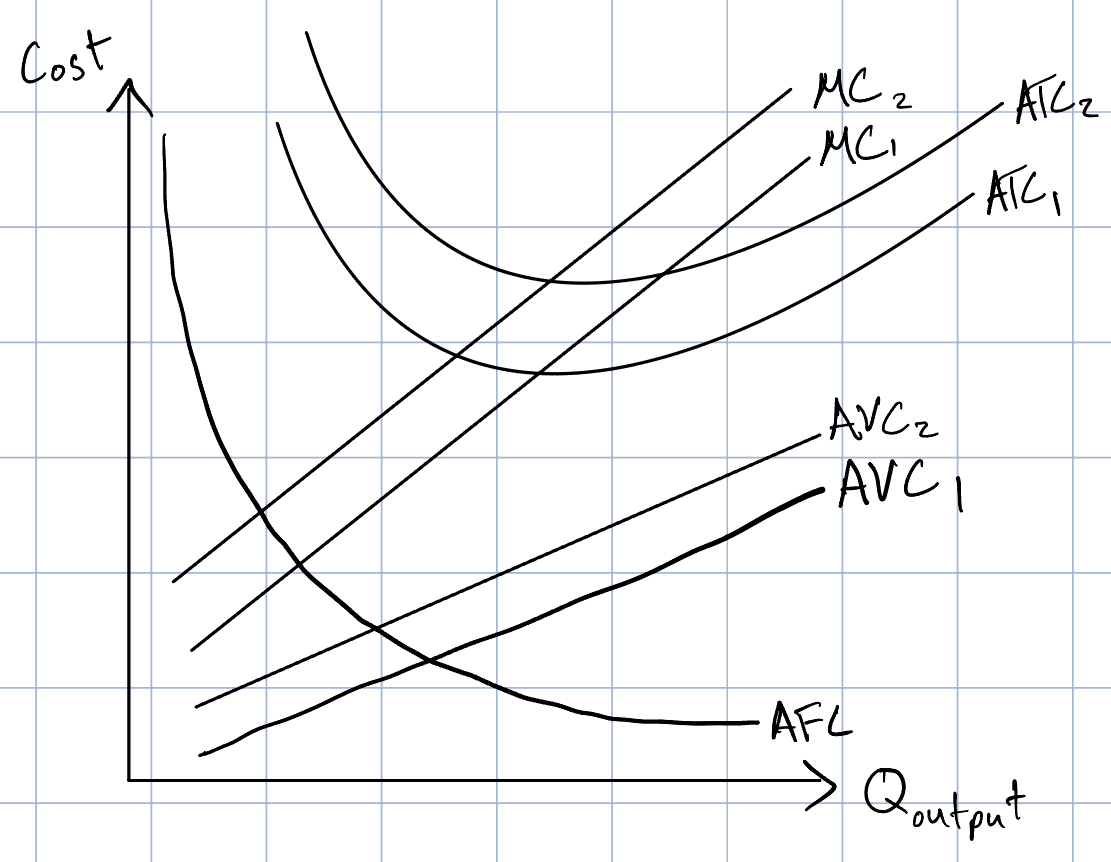
\includegraphics[width = 0.5\textwidth]{p6b}
		\end{center}
	
	\end{enumerate}
	
\item ATC: When MC is less than ATC, producing one more unit pulls ATC down, so ATC is decreasing. Similarly, when MC is greater than ATC, producing one more unit pulls ATC up, so ATC is increasing. Therefore, when MC intersects ATC, ATC switches from decreasing to increasing, so ATC is at a minimum.

AVC: When MC is greater than AVC, producing one more unit pulls AVC up, so AVC is increasing.

	\begin{enumerate}
	
	\item \phantom{x}
	
	\begin{center}
	\begin{tabular}{c | c | c | c | c | c}
	Quantity & VC & TC & AVC & ATC & MC\\
	\hline
	0 & 0 & 30 & -- & -- & -- \\
	1 & 10 & 40 & 10 & 40 & 10 \\
	2 & 25 & 55 & 12.5 & 27.5 & 15 \\
	3 & 45 & 75 & 15 & 25 & 20 \\
	4 & 70 & 100 & 17.5 & 25 & 25 \\
	5 & 100 & 130 & 20 & 26 & 30 \\
	6 & 135 & 165 & 22.5 & 27.5 & 35
	\end{tabular}
	\end{center}
	
	\end{enumerate}
	
\item Below is a table of each firm's ATC.

	\begin{center}
	\begin{tabular}{| c | c | c | c | c | c | c | c |}
	\hline
	\textbf{Quantity} & 1 & 2 & 3 & 4 & 5 & 6 & 7 \\
	\hline
	\textbf{Firm A} & \$60 & \$35 & \$26.67 & \$22.5 & \$20 & \$18.33 & \$17.14 \\
	\hline
	\textbf{Firm B} & 11 & 12 & 13 & 14 & 15 & 16 & 17 \\
	\hline
	\textbf{Firm C} & 21 & 17 & 16.33 & 16.5 & 17 & 17.67 & 18.43 \\
	\hline
	\end{tabular}
	\end{center}
	
	Firm A experiences economies of scale because their ATC decreases as their output increases. Firm B experiences diseconomies of scale because their ATC increases as their output increases. Firm C initially experiences economies of scale and then experiences diseconomies of scale.

\end{enumerate}

\end{document}